% ============================================================
%  Zero-Day IoT Attack Detection – Final Year Project Report
%  Central Institute of Technology Kokrajhar
% ============================================================
\documentclass[12pt,a4paper]{report}

% ── Packages ─────────────────────────────────────────────────
\usepackage[a4paper, left=1.5in, right=1in, top=1in, bottom=1in]{geometry}
\usepackage{graphicx}
\usepackage{booktabs}
\usepackage{array}
\usepackage{longtable}
\usepackage{multirow}
\usepackage{amsmath}
\usepackage{amssymb}
\usepackage{hyperref}
\usepackage{setspace}
\usepackage{fancyhdr}
\usepackage{titlesec}
\usepackage{caption}
\usepackage{subcaption}
\usepackage{float}
\usepackage{enumitem}
\usepackage{xcolor}
\usepackage{url}
\usepackage{cite}
\usepackage{microtype}
\usepackage{listings}
\usepackage{algorithm}
\usepackage{algpseudocode}
\usepackage{tocloft}
\usepackage{indentfirst}

% ── Hyperref setup ───────────────────────────────────────────
\hypersetup{
    colorlinks=true,
    linkcolor=black,
    citecolor=black,
    urlcolor=blue,
    pdftitle={Zero-Day IoT Attack Detection Using a Hybrid Machine Learning Approach},
    pdfauthor={Shahil Ahmed, Jagriti Shivam, Khushi Das, Babul Hoque}
}

% ── Line spacing ─────────────────────────────────────────────
\onehalfspacing

% ── Header / footer ──────────────────────────────────────────
\pagestyle{fancy}
\fancyhf{}
\fancyhead[L]{\small\leftmark}
\fancyhead[R]{\small CIT Kokrajhar}
\fancyfoot[C]{\thepage}
\renewcommand{\headrulewidth}{0.4pt}

% ── Chapter title formatting ─────────────────────────────────
\titleformat{\chapter}[display]
  {\normalfont\Large\bfseries\centering}
  {\chaptertitlename\ \thechapter}{10pt}{\huge}
\titlespacing*{\chapter}{0pt}{-10pt}{20pt}

% ── Code listing style ───────────────────────────────────────
\lstset{
  basicstyle=\ttfamily\small,
  breaklines=true,
  frame=single,
  numbers=left,
  numberstyle=\tiny,
  keywordstyle=\color{blue},
  commentstyle=\color{gray},
  stringstyle=\color{red}
}

% ── Graphics path ────────────────────────────────────────────
\graphicspath{{../../screenshots/}}

% ============================================================
\begin{document}

% ── Title page ───────────────────────────────────────────────
\begin{titlepage}
\centering
\vspace*{0.5cm}

{\Large\bfseries
Zero-Day IoT Attack Detection Using a\\[6pt]
Hybrid Machine Learning Approach\\[4pt]
(LightGBM + Autoencoder Fusion Model)
\par}

\vspace{0.6cm}
{\normalsize
A Project Work Submitted in Partial Fulfillment\\
of the requirements for the Degree\\[4pt]
\textit{BACHELOR OF TECHNOLOGY}\\[2pt]
in\\[2pt]
\textit{\textcolor{blue}{COMPUTER SCIENCE \& ENGINEERING}}
\par}

\vspace{0.5cm}
{\normalsize by\par}
\vspace{0.3cm}

{\normalsize
Shahil Ahmed \quad (Roll No. 202202021046)\\[4pt]
Jagriti Shivam \quad (Roll No. 202202021091)\\[4pt]
Khushi Das \quad\quad (Roll No. 202202021113)\\[4pt]
Babul Hoque \quad\quad (Roll No. 202202021020)
\par}

\vspace{0.5cm}
{\normalsize Under the Supervision of\par}
\vspace{0.2cm}
{\normalsize\bfseries Mr. Bikramjit Choudhury, Asst. Prof.\par}

\vspace{0.5cm}

\includegraphics[width=0.22\textwidth]{../../Project Report Template/cit_logo.png}
\par
\vspace{0.4cm}

{\normalsize\bfseries DEPARTMENT OF COMPUTER SCIENCE \& ENGINEERING\par}
\vspace{0.15cm}
{\small\textcolor{blue}{केन्द्रीय प्रौद्योगिकी संस्थान कोकराझार}\par}
\vspace{0.1cm}
{\normalsize CENTRAL INSTITUTE OF TECHNOLOGY KOKRAJHAR\par}
{\small (A Centrally Funded Institute under Ministry of HRD, Govt. of India)\\
BODOLAND TERRITORIAL AREAS DISTRICTS :: KOKRAJHAR :: ASSAM :: 783370\\
Website: www.cit.ac.in\par}
\vspace{0.3cm}
{\normalsize MAY 2026\par}
\end{titlepage}

% ── Certificate of Approval ──────────────────────────────────
\newpage
\thispagestyle{empty}
\begin{center}
{\Large\bfseries\underline{CERTIFICATE OF APPROVAL}}
\end{center}
\vspace{1cm}

\noindent This is to certify that the work embodied in this project entitled
\textbf{Zero-Day IoT Attack Detection Using a Hybrid Machine Learning Approach}
submitted by \textbf{Shahil Ahmed, Jagriti Shivam, Khushi Das,} and \textbf{Babul Hoque}
to the Department of Computer Science \& Engineering, is carried out under our direct
supervision and guidance.

\vspace{0.5cm}
\noindent The project work has been prepared as per the regulations of Central Institute
of Technology and I strongly recommend that this project work be accepted in partial
fulfillment of the requirement for the degree of B.Tech in Computer Science and Engineering.

\vspace{3cm}
\noindent\textbf{Supervisor}

\vspace{1.5cm}
\noindent\textbf{(Mr. Bikramjit Choudhury)}\\
Asst. Prof., Dept. of CSE

% ── Certificate by Board of Examiners ───────────────────────
\newpage
\thispagestyle{empty}
\begin{center}
{\Large\bfseries\underline{Certificate by the Board of Examiners}}
\end{center}
\vspace{1cm}

\noindent This is to certify that the project work entitled
\textbf{Zero-Day IoT Attack Detection Using a Hybrid Machine Learning Approach}
submitted by \textbf{Shahil Ahmed, Jagriti Shivam, Khushi Das,} and \textbf{Babul Hoque}
to the Department of Computer Science and Engineering of Central Institute of Technology,
Kokrajhar has been examined and evaluated.

\vspace{0.5cm}
\noindent The project work has been prepared as per the regulations of Central Institute
of Technology and qualifies to be accepted in partial fulfillment of the requirement for
the degree of B.Tech in Computer Science and Engineering.

\vspace{2.5cm}
\noindent Project Co-ordinator

\vspace{2.5cm}
\noindent Countersigned by

\vspace{1.5cm}
\noindent\textbf{(Dr. Faculty Name)}\\
\textbf{HoD}\\
Department of CSE

% ── Acknowledgement ──────────────────────────────────────────
\newpage
\thispagestyle{empty}
\begin{center}
{\Large\bfseries\underline{ACKNOWLEDGEMENT}}
\end{center}
\vspace{1cm}

\noindent We would like to express our sincere gratitude to
\textbf{Mr. Bikramjit Choudhury}, Assistant Professor, Department of Computer Science \&
Engineering, Central Institute of Technology Kokrajhar, for his invaluable guidance,
constant encouragement, and constructive suggestions throughout the course of this project.
His expertise in machine learning and network security significantly shaped the direction
and quality of this work.

\vspace{0.5cm}
\noindent We are thankful to the \textbf{Head of the Department} and all the faculty members
of the Department of CSE, CIT Kokrajhar, for providing us with the resources and academic
environment necessary to carry out this project.

\vspace{0.5cm}
\noindent We are also grateful to the creators of the
\textbf{Edge-IIoTset} dataset~\cite{dataset_edge_iiotset} for making it publicly available,
which formed the backbone of our experimental evaluation.

\vspace{0.5cm}
\noindent Finally, we acknowledge the contributions of the open-source community behind
the Python libraries — \texttt{scikit-learn}, \texttt{LightGBM}, \texttt{TensorFlow/Keras},
and \texttt{Pandas} — that powered our implementation.

\vspace{1.5cm}
\noindent Date: \underline{\hspace{3cm}}
\hfill
\begin{tabular}{l}
Shahil Ahmed \quad (202202021046)\\[6pt]
Jagriti Shivam \quad (202202021091)\\[6pt]
Khushi Das \quad\quad (202202021113)\\[6pt]
Babul Hoque \quad\quad (202202021020)
\end{tabular}

% ── Abstract ─────────────────────────────────────────────────
\newpage
\begin{center}
{\Large\bfseries ABSTRACT}
\end{center}
\addcontentsline{toc}{chapter}{Abstract}
\vspace{0.5cm}

The rapid proliferation of Internet of Things (IoT) devices has introduced significant
cybersecurity challenges. While traditional intrusion detection systems perform well
against known attacks, they fail to detect novel or zero-day threats — attacks that
have never been seen before. This project proposes and implements a \textbf{hybrid
intrusion detection system (IDS)} for IoT networks that combines a supervised classifier
and an unsupervised anomaly detector to address both known and zero-day attacks.

\vspace{0.5cm}
\noindent The proposed system leverages the \textbf{Edge-IIoTset} dataset, a comprehensive
IoT network traffic dataset containing 15 attack categories. We adopt a two-stage pipeline:
first, a \textbf{LightGBM} classifier is trained on 10 known attack types to achieve
high-accuracy classification of familiar threats (99.99\%); second, a symmetric
\textbf{Autoencoder} neural network is trained exclusively on normal traffic to
reconstruct-error-based anomaly detection of zero-day attacks (99.19\% accuracy on
the full dataset). A \textbf{Fusion Model} integrates both components using a confidence-based
routing strategy, achieving 96.82\% accuracy on a combined test set including
five previously unseen zero-day attack categories.

\vspace{0.5cm}
\noindent Experimental results demonstrate that the proposed hybrid approach significantly
outperforms baseline methods such as Isolation Forest (49\% accuracy), confirming the
effectiveness of combining supervised and unsupervised techniques for robust IoT
intrusion detection.

\vspace{0.5cm}
\noindent \textbf{Keywords:} IoT Security, Intrusion Detection, Zero-Day Attacks, LightGBM,
Autoencoder, Anomaly Detection, Fusion Model, Edge-IIoTset.

% ── Table of Contents ────────────────────────────────────────
\newpage
\tableofcontents

% ── List of Figures ──────────────────────────────────────────
\newpage
\listoffigures
\addcontentsline{toc}{chapter}{List of Figures}

% ── List of Tables ───────────────────────────────────────────
\newpage
\listoftables
\addcontentsline{toc}{chapter}{List of Tables}

\newpage
\pagenumbering{arabic}


% ============================================================
%  CHAPTER 1 – INTRODUCTION
% ============================================================
\chapter{Introduction}

\section{Background}

The Internet of Things (IoT) refers to the interconnected network of physical
devices — sensors, actuators, embedded computers, and smart appliances — that
communicate over the internet to exchange data and perform automated tasks.
As of 2024, there are an estimated 15 billion active IoT devices worldwide,
with projections exceeding 30 billion by 2030~\cite{iot_growth}. These devices
span critical sectors including healthcare, industrial automation, smart grids,
transportation, and home automation.

\noindent However, the expanding IoT ecosystem has dramatically widened the
cybersecurity attack surface. IoT devices are typically resource-constrained
(limited CPU, memory, and battery), run outdated firmware, lack encryption,
and are often deployed without proper security configuration. This makes them
prime targets for cyber attackers who exploit vulnerabilities to launch
Distributed Denial of Service (DDoS) attacks, data exfiltration campaigns,
ransomware, and network intrusions~\cite{iot_security_challenges}.

\section{Problem Statement}

Traditional signature-based intrusion detection systems (IDS) rely on
pre-defined patterns of known attacks. While effective against familiar
threats, they are fundamentally incapable of detecting \textbf{zero-day
attacks} — novel intrusions that exploit previously unknown vulnerabilities
or employ new attack strategies never seen in training data.

\noindent The key challenges addressed in this project are:
\begin{enumerate}
  \item \textbf{Known Attack Detection}: Accurately classifying network
        traffic among multiple known attack categories in real time.
  \item \textbf{Zero-Day Detection}: Identifying anomalous traffic that does
        not match any known attack pattern.
  \item \textbf{Integration}: Building a unified system that handles both
        known and zero-day threats simultaneously.
\end{enumerate}

\section{Objectives}

The primary objectives of this project are:
\begin{itemize}
  \item To design and implement a hybrid intrusion detection framework
        combining supervised and unsupervised machine learning.
  \item To evaluate the effectiveness of LightGBM for classifying known
        IoT attack types.
  \item To train and evaluate an Autoencoder for zero-day anomaly detection
        based on reconstruction error.
  \item To develop a Fusion Model that integrates both approaches using a
        confidence-based routing mechanism.
  \item To benchmark the proposed system against baseline methods including
        Isolation Forest.
\end{itemize}

\section{Scope of Work}

This project uses the Edge-IIoTset dataset~\cite{dataset_edge_iiotset},
a publicly available IoT network traffic dataset. The scope includes:
\begin{itemize}
  \item Data preprocessing and feature engineering on real IoT network captures.
  \item Training and evaluation of LightGBM on 10 known attack categories.
  \item Training an Autoencoder exclusively on normal traffic for anomaly detection.
  \item Building a fusion pipeline that routes traffic based on classifier confidence.
  \item Full experimental evaluation with classification reports, confusion matrices,
        and comparative accuracy analysis.
\end{itemize}

\section{Report Organisation}

The remainder of this report is organised as follows:
\begin{itemize}
  \item \textbf{Chapter 2} presents a review of related work in IoT security,
        intrusion detection, and anomaly-based detection.
  \item \textbf{Chapter 3} describes the system design including the dataset,
        preprocessing pipeline, and architectural overview.
  \item \textbf{Chapter 4} details the implementation of each component.
  \item \textbf{Chapter 5} presents experimental results and evaluation.
  \item \textbf{Chapter 6} discusses findings, limitations, and future work.
  \item \textbf{Chapter 7} concludes the report.
\end{itemize}



% ============================================================
%  CHAPTER 2 – LITERATURE REVIEW
% ============================================================
\chapter{Literature Review}

\section{IoT Security Landscape}

The IoT security problem has attracted significant academic attention over
the past decade. Pa et al.~\cite{iot_malware} demonstrated that IoT devices
are regularly infected by malware such as Mirai, which exploits default
credentials to build large-scale botnets. The Mirai botnet attack of 2016
disrupted major internet infrastructure and highlighted the systemic
vulnerability of IoT ecosystems~\cite{mirai_attack}.

\noindent Network intrusion detection systems (NIDS) have traditionally used
two paradigms: \textbf{signature-based} detection and \textbf{anomaly-based}
detection~\cite{nids_survey}. Signature-based systems match traffic against a
database of known attack patterns; they achieve high precision but fail entirely
against zero-day attacks. Anomaly-based systems model normal behaviour and flag
deviations, providing zero-day capability at the cost of higher false positive rates.

\section{Machine Learning for Intrusion Detection}

The application of machine learning to network intrusion detection has grown
substantially. Random Forests and ensemble methods were among the first ML
approaches applied to IDS, showing strong performance on benchmark datasets
such as KDD Cup 1999~\cite{kdd_cup}. More recently, gradient boosting frameworks
have surpassed older methods.

\noindent \textbf{LightGBM}~\cite{lightgbm_paper}, proposed by Ke et al. (2017),
is a gradient boosting framework that uses histogram-based algorithms and
leaf-wise tree growth, achieving state-of-the-art performance on tabular
classification tasks with lower memory usage and faster training than XGBoost.
Several studies have applied LightGBM to network traffic classification with
excellent results~\cite{lgbm_ids}.

\section{Autoencoders for Anomaly Detection}

Autoencoders are neural networks trained to compress and reconstruct their
input~\cite{autoencoder_original}. When trained only on normal data, they learn
a compact representation of normality. Anomalous inputs produce high reconstruction
errors, which serve as anomaly scores. This principle has been applied widely in
fraud detection~\cite{ae_fraud}, medical anomaly detection~\cite{ae_medical},
and network intrusion detection~\cite{ae_ids}.

\noindent Schlegl et al.~\cite{ganomaly} and Zenati et al.~\cite{efficient_gan}
extended the concept using GANs for anomaly detection. However, standard
autoencoders remain competitive for tabular network data due to their simplicity
and interpretability.

\section{Hybrid Approaches}

Hybrid IDS combining supervised and unsupervised components have been explored
to address the limitations of each individually. Yin et al.~\cite{hybrid_ids}
proposed combining deep neural networks with anomaly detectors for intrusion
detection. Similarly, Khraisat et al.~\cite{hybrid_survey} surveyed hybrid IDS
architectures and found that combining multiple detection paradigms consistently
outperforms single-model approaches.

\noindent The key insight motivating this project is that a supervised classifier
can achieve near-perfect accuracy on known attacks, while an unsupervised anomaly
detector handles novel threats — and the two can be fused via a confidence-based
routing mechanism to achieve robust end-to-end coverage.

\section{IoT-Specific Datasets}

The lack of realistic, labelled IoT network datasets was a major bottleneck
in IDS research until recently. The \textbf{Edge-IIoTset} dataset~\cite{dataset_edge_iiotset},
created by Ferrag et al. (2022), addressed this gap by providing a comprehensive
benchmark collected from a realistic IoT testbed including 10 types of IoT devices
and 15 categories of attacks spanning DDoS, reconnaissance, injection, and malware
attacks. This dataset is used in the present work.



% ============================================================
%  CHAPTER 3 – SYSTEM DESIGN
% ============================================================
\chapter{System Design}

\section{Overview of Proposed Architecture}

The proposed hybrid Intrusion Detection System (IDS) consists of three
functional components arranged in a sequential pipeline:

\begin{enumerate}
  \item \textbf{Preprocessing Module}: Cleans and normalises raw network
        traffic data into a feature matrix suitable for ML models.
  \item \textbf{LightGBM Classifier}: A supervised multiclass classifier
        trained on 10 known attack categories to distinguish between
        different known threat types.
  \item \textbf{Autoencoder Anomaly Detector}: An unsupervised neural network
        trained exclusively on normal traffic that flags inputs with
        high reconstruction error as anomalous (potential zero-day attacks).
  \item \textbf{Fusion Model}: A decision-level fusion layer that routes
        traffic predictions using a confidence threshold strategy:
        if LightGBM assigns $\geq$90\% confidence to ``Normal'', the
        traffic is classified as normal; otherwise, the Autoencoder
        makes the final decision.
\end{enumerate}

\begin{figure}[H]
  \centering
  \fbox{\parbox{0.85\textwidth}{\centering\vspace{0.3cm}
  \textbf{System Architecture (Conceptual Flow)}\\[8pt]
  Raw IoT Traffic $\rightarrow$ Preprocessing $\rightarrow$
  \begin{tabular}{c}LightGBM\\(Known Attacks)\end{tabular}
  + \begin{tabular}{c}Autoencoder\\(Zero-Day)\end{tabular}
  $\rightarrow$ Fusion Model $\rightarrow$ Classification Output
  \vspace{0.3cm}}}
  \caption{High-level architecture of the proposed hybrid IDS}
  \label{fig:architecture}
\end{figure}

\section{Dataset Description}

\subsection{Edge-IIoTset}

The \textbf{Edge-IIoTset} dataset~\cite{dataset_edge_iiotset} is used
in this work. It was created from a realistic IoT testbed running
10 types of IoT devices including cameras, temperature sensors, weather
stations, and smart home appliances. Network traffic was captured using
Wireshark and includes both benign traffic and 14 categories of attacks.

\subsubsection{Dataset Statistics}

\begin{itemize}
  \item \textbf{Original size}: 157,800 rows $\times$ 63 features
  \item \textbf{After cleaning}: 152,389 rows $\times$ 53 features
  \item \textbf{Protocols covered}: TCP, UDP, ICMP, HTTP, MQTT, DNS, ARP,
        Modbus TCP
\end{itemize}

\subsubsection{Attack Categories}

The dataset contains 15 traffic categories (1 normal + 14 attacks):

\begin{table}[H]
\centering
\caption{Attack categories in Edge-IIoTset and their classification}
\label{tab:attack_categories}
\begin{tabular}{clll}
\toprule
\textbf{ID} & \textbf{Attack Type} & \textbf{Protocol/Vector} & \textbf{Split} \\
\midrule
0  & Normal              & —                    & Known (train) \\
1  & Backdoor            & Malware              & Known (train) \\
2  & DDoS\_HTTP          & HTTP flood           & Known (train) \\
3  & DDoS\_ICMP          & ICMP flood           & Known (train) \\
4  & DDoS\_TCP           & TCP flood            & Known (train) \\
5  & DDoS\_UDP           & UDP flood            & Known (train) \\
6  & SQL\_Injection       & Application          & Known (train) \\
7  & Uploading           & Exfiltration         & Known (train) \\
8  & Vulnerability\_Scanner & Reconnaissance    & Known (train) \\
9  & Password Attack      & Brute force         & Known (train) \\
\midrule
10 & Ransomware          & Malware              & Zero-day (test) \\
11 & XSS                 & Web                  & Zero-day (test) \\
12 & Port\_Scanning       & Reconnaissance      & Zero-day (test) \\
13 & Fingerprinting      & Reconnaissance       & Zero-day (test) \\
14 & MITM                & Network interception & Zero-day (test) \\
\bottomrule
\end{tabular}
\end{table}

\subsection{Data Split Strategy}

The dataset is partitioned into two non-overlapping subsets:
\begin{itemize}
  \item \textbf{Known training set}: 10 traffic classes (Normal + 9 attacks),
        totalling 121,293 samples. Used to train the LightGBM classifier.
  \item \textbf{Zero-day test set}: 5 unseen attack categories, totalling
        31,096 samples. Used exclusively to evaluate the Fusion Model.
\end{itemize}

\noindent Critically, no zero-day attack traffic is included in the training
phase of any component. This setup rigorously simulates a real-world scenario
where the system must detect attacks it has never encountered.

\section{Preprocessing Pipeline}

The raw dataset requires significant preprocessing before use:

\begin{enumerate}
  \item \textbf{Column removal}: 10 high-cardinality or irrelevant columns
        are dropped (e.g., frame timestamps, IP addresses, HTTP URIs).
  \item \textbf{Missing value handling}: Rows with null values are removed.
  \item \textbf{Duplicate removal}: Duplicate records are eliminated.
        This reduces the dataset from 157,800 to 152,389 rows.
  \item \textbf{Categorical encoding}: String-typed columns (HTTP method,
        TCP flags, MQTT fields) are label-encoded to integers.
  \item \textbf{Datatype casting}: All features are cast to \texttt{float32}
        or \texttt{int32} to reduce memory footprint.
  \item \textbf{Feature scaling}: A \texttt{StandardScaler} is fitted
        \emph{exclusively on normal traffic} to normalise features for
        Autoencoder training. This ensures the scaler learns only the
        distribution of benign activity.
\end{enumerate}

\section{LightGBM Classifier Design}

LightGBM (Light Gradient Boosting Machine)~\cite{lightgbm_paper} is
selected for supervised classification due to its:
\begin{itemize}
  \item Superior speed on large tabular datasets.
  \item Native support for multiclass classification.
  \item Low memory footprint.
  \item Strong generalisation with minimal hyperparameter tuning.
\end{itemize}

\noindent The classifier is configured with the following hyperparameters:
\begin{table}[H]
\centering
\caption{LightGBM hyperparameter configuration}
\label{tab:lgbm_params}
\begin{tabular}{ll}
\toprule
\textbf{Hyperparameter} & \textbf{Value} \\
\midrule
\texttt{n\_estimators}   & 300 \\
\texttt{learning\_rate}  & 0.05 \\
\texttt{max\_depth}      & 10 \\
\texttt{num\_leaves}     & 50 \\
\texttt{objective}       & multiclass \\
\texttt{num\_class}      & 10 \\
\texttt{random\_state}   & 42 \\
\bottomrule
\end{tabular}
\end{table}

\section{Autoencoder Design}

The Autoencoder is a symmetric fully-connected neural network:

\begin{table}[H]
\centering
\caption{Autoencoder architecture}
\label{tab:ae_arch}
\begin{tabular}{cll}
\toprule
\textbf{Layer} & \textbf{Units} & \textbf{Activation} \\
\midrule
Input           & 51  & — \\
Encoder Dense 1 & 64  & ReLU \\
Encoder Dense 2 & 32  & ReLU \\
Bottleneck      & 16  & ReLU \\
Decoder Dense 1 & 32  & ReLU \\
Decoder Dense 2 & 64  & ReLU \\
Output          & 51  & Linear \\
\midrule
\multicolumn{2}{l}{Total trainable parameters} & 11,907 \\
\bottomrule
\end{tabular}
\end{table}

\noindent \textbf{Training procedure}:
\begin{itemize}
  \item Trained exclusively on normal traffic (24,152 samples).
  \item 80/20 split: 19,321 training / 4,831 validation samples.
  \item Loss function: Mean Squared Error (MSE).
  \item Optimiser: Adam.
  \item Early stopping: patience = 5 epochs; training stopped at epoch 45.
\end{itemize}

\noindent \textbf{Anomaly threshold}: The reconstruction error threshold
is set at the \textbf{95th percentile} of validation reconstruction errors:
\begin{equation}
  \tau = \text{Percentile}_{95}(\{\|x_i - \hat{x}_i\|^2 : x_i \in X_{\text{val}}\})
  = 0.01218
\end{equation}
Traffic with reconstruction error $> \tau$ is classified as anomalous.

\section{Fusion Model Design}

The Fusion Model integrates LightGBM and the Autoencoder using the
following decision logic:

\begin{algorithm}[H]
\caption{Fusion Model Decision Logic}
\label{alg:fusion}
\begin{algorithmic}[1]
\Require Input traffic sample $x$
\Ensure Classification label $y$
\State Compute LightGBM softmax probabilities: $p = \text{LightGBM}(x)$
\State $p_{\text{normal}} = p[\text{class=Normal}]$
\If{$p_{\text{normal}} \geq 0.90$}
    \State $y \leftarrow \text{Normal}$
\Else
    \State Compute reconstruction error: $e = \|x - \text{Autoencoder}(x)\|^2$
    \If{$e > \tau$}
        \State $y \leftarrow \text{Attack (Anomaly)}$
    \Else
        \State $y \leftarrow \text{Normal}$
    \EndIf
\EndIf
\Return $y$
\end{algorithmic}
\end{algorithm}

\noindent This strategy ensures that LightGBM handles high-confidence
known-traffic decisions, while the Autoencoder is invoked for borderline
or unfamiliar traffic, enabling zero-day detection.



% ============================================================
%  CHAPTER 4 – IMPLEMENTATION
% ============================================================
\chapter{Implementation}

\section{Development Environment}

The project was implemented in Python 3 using the following libraries:

\begin{table}[H]
\centering
\caption{Software stack and dependencies}
\label{tab:software}
\begin{tabular}{ll}
\toprule
\textbf{Library} & \textbf{Purpose} \\
\midrule
Python 3.10+       & Core programming language \\
Pandas             & Data loading and manipulation \\
NumPy              & Numerical computation \\
Scikit-learn       & Preprocessing, metrics, Isolation Forest \\
LightGBM 4.x       & Supervised gradient boosting classifier \\
TensorFlow / Keras & Autoencoder neural network \\
Matplotlib         & Visualisation \\
Seaborn            & Heatmaps and confusion matrices \\
KaggleHub          & Dataset download (Edge-IIoTset) \\
Google Colab       & Cloud GPU execution environment \\
\bottomrule
\end{tabular}
\end{table}

\noindent All Jupyter notebooks were executed on Google Colab with GPU
acceleration. Model artefacts (trained weights, scaler, threshold) were
persisted to Google Drive and then exported to the project repository.

\section{Notebook Pipeline}

The implementation is structured across five Jupyter notebooks:

\begin{table}[H]
\centering
\caption{Notebook pipeline structure}
\label{tab:notebooks}
\begin{tabular}{clp{8cm}}
\toprule
\textbf{Notebook} & \textbf{Name} & \textbf{Description} \\
\midrule
01 & Preprocessing Master       & Downloads dataset, cleans, encodes, splits, fits scaler \\
02 & Known Attack LightGBM      & Trains and evaluates LightGBM on 10 known classes \\
03 & Zero-Day Autoencoder       & Trains Autoencoder on normal traffic, sets threshold \\
04 & Fusion Model               & Combines LightGBM + Autoencoder via confidence routing \\
05 & Visualisation \& Comparison & Plots comparative charts and final summaries \\
\bottomrule
\end{tabular}
\end{table}

\section{Preprocessing Implementation}

The preprocessing notebook performs the following steps:

\begin{lstlisting}[language=Python, caption={Key preprocessing steps}]
import pandas as pd
from sklearn.preprocessing import StandardScaler, LabelEncoder
import pickle

# Load dataset
df = pd.read_csv('ML-EdgeIIoT-dataset.csv', low_memory=False)

# Drop irrelevant columns
drop_cols = ['frame.time', 'ip.src_host', 'ip.dst_host',
             'arp.src.proto_ipv4', 'arp.dst.proto_ipv4',
             'http.file_data', 'http.request.full_uri', ...]
df.drop(columns=drop_cols, inplace=True)

# Clean nulls and duplicates
df.dropna(inplace=True)
df.drop_duplicates(inplace=True)

# Label encode categorical columns
for col in df.select_dtypes(include='object').columns:
    df[col] = LabelEncoder().fit_transform(df[col])

# Downcast dtypes
df = df.astype('float32')

# Fit StandardScaler on NORMAL traffic only
normal_df = df[df['Attack_label'] == 0].drop(columns=['Attack_label', ...])
scaler = StandardScaler()
scaler.fit(normal_df)
pickle.dump(scaler, open('scaler.pkl', 'wb'))
\end{lstlisting}

\section{LightGBM Training}

\begin{lstlisting}[language=Python, caption={LightGBM training}]
import lightgbm as lgb
from sklearn.model_selection import train_test_split

# Load known training data
known_df = pd.read_parquet('known_train.parquet')
X = known_df.drop(columns=['Attack_type'])
y = known_df['Attack_type']

# 80/20 stratified split
X_train, X_test, y_train, y_test = train_test_split(
    X, y, test_size=0.2, stratify=y, random_state=42)

# Train LightGBM
clf = lgb.LGBMClassifier(
    n_estimators=300, learning_rate=0.05,
    max_depth=10, num_leaves=50,
    objective='multiclass', random_state=42)
clf.fit(X_train, y_train)
\end{lstlisting}

\section{Autoencoder Training}

\begin{lstlisting}[language=Python, caption={Autoencoder architecture and training}]
from tensorflow.keras import layers, models, callbacks
import numpy as np

# Build Autoencoder
inputs = layers.Input(shape=(51,))
x = layers.Dense(64, activation='relu')(inputs)
x = layers.Dense(32, activation='relu')(x)
encoded = layers.Dense(16, activation='relu')(x)
x = layers.Dense(32, activation='relu')(encoded)
x = layers.Dense(64, activation='relu')(x)
outputs = layers.Dense(51)(x)
autoencoder = models.Model(inputs, outputs)
autoencoder.compile(optimizer='adam', loss='mse')

# Train on normal traffic only
es = callbacks.EarlyStopping(patience=5, restore_best_weights=True)
autoencoder.fit(X_normal_train, X_normal_train,
                epochs=50, batch_size=256,
                validation_data=(X_normal_val, X_normal_val),
                callbacks=[es])

# Set anomaly threshold at 95th percentile of val reconstruction error
val_preds = autoencoder.predict(X_normal_val)
val_errors = np.mean(np.square(X_normal_val - val_preds), axis=1)
threshold = np.percentile(val_errors, 95)  # = 0.01218
\end{lstlisting}

\section{Fusion Model Implementation}

\begin{lstlisting}[language=Python, caption={Fusion Model prediction logic}]
def fusion_predict(X_scaled, X_raw):
    """
    X_scaled: Autoencoder-scaled features
    X_raw:    Raw features for LightGBM
    Returns binary labels: 0=Normal, 1=Attack
    """
    predictions = []
    lgb_probs = clf.predict_proba(X_raw)

    for i in range(len(X_raw)):
        normal_conf = lgb_probs[i, class_to_idx['Normal']]

        if normal_conf >= 0.90:
            predictions.append(0)  # Normal
        else:
            # Defer to Autoencoder
            sample = X_scaled[i].reshape(1, -1)
            recon = autoencoder.predict(sample, verbose=0)
            error = np.mean(np.square(sample - recon))
            predictions.append(1 if error > threshold else 0)

    return np.array(predictions)
\end{lstlisting}

\section{Saved Model Artefacts}

The trained models are persisted for reproducibility:

\begin{table}[H]
\centering
\caption{Saved model artefacts}
\label{tab:artefacts}
\begin{tabular}{lll}
\toprule
\textbf{File} & \textbf{Format} & \textbf{Description} \\
\midrule
\texttt{lightgbm\_known.pkl}  & Pickle  & Trained LightGBM classifier \\
\texttt{autoencoder.keras}    & Keras   & Trained Autoencoder weights \\
\texttt{scaler.pkl}           & Pickle  & StandardScaler fitted on normal traffic \\
\texttt{ae\_threshold.pkl}    & Pickle  & Reconstruction error threshold (0.01218) \\
\bottomrule
\end{tabular}
\end{table}



% ============================================================
%  CHAPTER 5 – RESULTS AND EVALUATION
% ============================================================
\chapter{Results and Evaluation}

\section{Experimental Setup}

All experiments were conducted on Google Colab (Tesla T4 GPU, 12 GB RAM).
Each model was evaluated on a held-out test set that was never seen
during training. Evaluation metrics include:
\begin{itemize}
  \item \textbf{Accuracy}: Overall fraction of correctly classified samples.
  \item \textbf{Precision}: Fraction of predicted positives that are truly positive.
  \item \textbf{Recall}: Fraction of actual positives correctly predicted.
  \item \textbf{F1-Score}: Harmonic mean of precision and recall.
  \item \textbf{Confusion Matrix}: Per-class visual breakdown of predictions.
\end{itemize}

\section{LightGBM Results}

\subsection{Accuracy}

The LightGBM classifier was trained on 97,034 samples across 10 classes
and evaluated on 24,259 test samples. It achieved an overall accuracy of
\textbf{99.99\%}.

\begin{figure}[H]
  \centering
  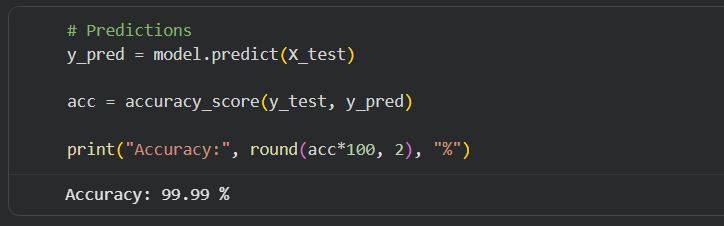
\includegraphics[width=0.85\textwidth]{LightGBM/Accuracy.png}
  \caption{LightGBM overall test accuracy}
  \label{fig:lgbm_accuracy}
\end{figure}

\subsection{Classification Report}

\begin{table}[H]
\centering
\caption{LightGBM per-class classification report (test set, n=24,259)}
\label{tab:lgbm_report}
\begin{tabular}{lcccc}
\toprule
\textbf{Class} & \textbf{Precision} & \textbf{Recall} & \textbf{F1-Score} & \textbf{Support} \\
\midrule
Backdoor (0)               & 1.0000 & 0.9995 & 0.9997 & 1,973 \\
DDoS\_HTTP (1)             & 1.0000 & 1.0000 & 1.0000 & 2,112 \\
DDoS\_ICMP (2)             & 1.0000 & 1.0000 & 1.0000 & 2,619 \\
DDoS\_TCP (3)              & 1.0000 & 1.0000 & 1.0000 & 2,049 \\
DDoS\_UDP (4)              & 1.0000 & 1.0000 & 1.0000 & 2,900 \\
Normal (7)                 & 1.0000 & 1.0000 & 1.0000 & 4,831 \\
Password (8)               & 0.9995 & 1.0000 & 0.9997 & 1,996 \\
SQL\_Injection (9)         & 0.9994 & 1.0000 & 0.9997 & 1,784 \\
Uploading (10)             & 0.9995 & 1.0000 & 0.9997 & 1,938 \\
Vulnerability\_Scanner (11)& 1.0000 & 1.0000 & 1.0000 & 2,057 \\
\midrule
\textbf{Weighted Avg}      & \textbf{0.9999} & \textbf{0.9999} & \textbf{0.9999} & \textbf{24,259} \\
\bottomrule
\end{tabular}
\end{table}

\begin{figure}[H]
  \centering
  
\includegraphics[width=0.85\textwidth]{LightGBM/Classification Report.png}
  \caption{LightGBM classification report (screenshot from Colab)}
  \label{fig:lgbm_clf_report}
\end{figure}

\subsection{Confusion Matrix}

\begin{figure}[H]
  \centering
  
\includegraphics[width=0.75\textwidth]{LightGBM/Confusion Matrix.png}
  \caption{LightGBM confusion matrix on 10-class test set}
  \label{fig:lgbm_cm}
\end{figure}

\noindent The confusion matrix confirms near-perfect separation across all
10 classes. The few misclassifications occur exclusively within attack categories
that share network-level characteristics (e.g., Password and SQL Injection).

\section{Autoencoder Results}

\subsection{Reconstruction Error and Threshold}

\begin{figure}[H]
  \centering
  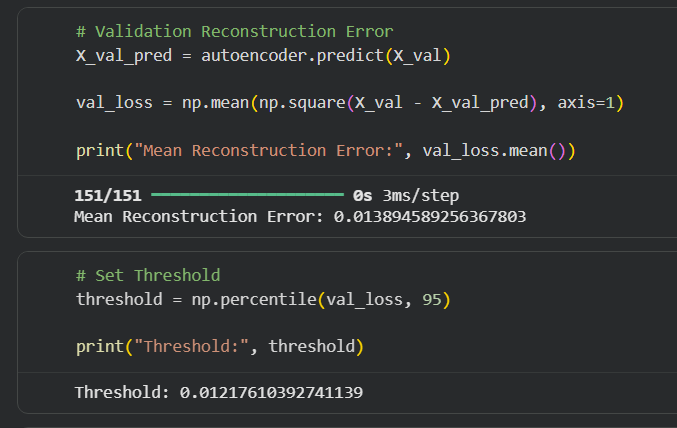
\includegraphics[width=0.85\textwidth]{Autoencoder/Reconstruction error & Threshold.png}
  \caption{Autoencoder reconstruction error distribution with anomaly threshold}
  \label{fig:ae_threshold}
\end{figure}

\noindent The figure shows the distribution of reconstruction errors on the
validation set. Normal traffic produces consistently low errors, while attack
traffic (applied retrospectively) produces higher errors. The threshold
$\tau = 0.01218$ (95th percentile of normal validation errors) cleanly
separates the two distributions.

\subsection{Classification Report}

The Autoencoder was evaluated in binary mode (Normal vs. Attack) on the
full 152,389-sample dataset:

\begin{table}[H]
\centering
\caption{Autoencoder binary classification report (full dataset, n=152,389)}
\label{tab:ae_report}
\begin{tabular}{lcccc}
\toprule
\textbf{Class} & \textbf{Precision} & \textbf{Recall} & \textbf{F1-Score} & \textbf{Support} \\
\midrule
Normal (0) & 1.0000 & 0.9487 & 0.9737 & 24,152 \\
Attack (1) & 0.9904 & 1.0000 & 0.9952 & 128,237 \\
\midrule
\textbf{Accuracy} & \multicolumn{4}{c}{\textbf{99.19\%}} \\
\textbf{Macro Avg} & 0.9952 & 0.9744 & 0.9844 & 152,389 \\
\textbf{Weighted Avg} & 0.9919 & 0.9919 & 0.9918 & 152,389 \\
\bottomrule
\end{tabular}
\end{table}

\begin{figure}[H]
  \centering
  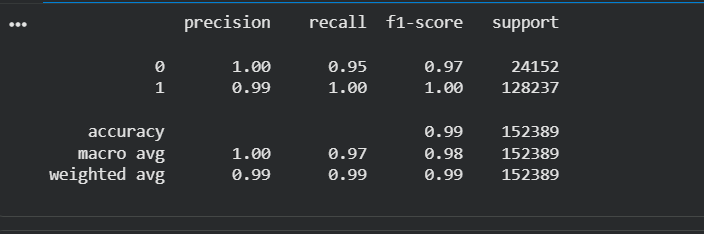
\includegraphics[width=0.80\textwidth]{Autoencoder/Classification Report.png}
  \caption{Autoencoder classification report (screenshot from Colab)}
  \label{fig:ae_clf_report}
\end{figure}

\subsection{Autoencoder Confusion Matrix}

\begin{figure}[H]
  \centering
  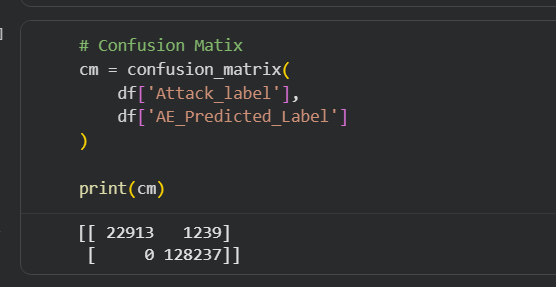
\includegraphics[width=0.70\textwidth]{Autoencoder/Confusion Matrix.png}
  \caption{Autoencoder confusion matrix (binary: Normal vs. Attack)}
  \label{fig:ae_cm}
\end{figure}

\noindent The Autoencoder achieves 100\% attack recall — it never misses an
attack. The 5.13\% false positive rate (1,239 normal samples classified as
attacks) represents the cost of this high sensitivity.

\section{Fusion Model Results}

\subsection{Test Configuration}

The Fusion Model is evaluated on a combined test set of:
\begin{itemize}
  \item \textbf{24,152} normal traffic samples
  \item \textbf{31,096} zero-day attack samples (5 unseen categories)
  \item \textbf{Total: 55,248 samples}
\end{itemize}

\subsection{Classification Report}

\begin{table}[H]
\centering
\caption{Fusion Model binary classification report (zero-day test set, n=55,248)}
\label{tab:fusion_report}
\begin{tabular}{lcccc}
\toprule
\textbf{Class} & \textbf{Precision} & \textbf{Recall} & \textbf{F1-Score} & \textbf{Support} \\
\midrule
Normal (0) & 0.9778 & 0.9487 & 0.9630 & 24,152 \\
Attack (1) & 0.9611 & 0.9833 & 0.9720 & 31,096 \\
\midrule
\textbf{Accuracy} & \multicolumn{4}{c}{\textbf{96.82\%}} \\
\textbf{Macro Avg} & 0.9694 & 0.9660 & 0.9675 & 55,248 \\
\textbf{Weighted Avg} & 0.9684 & 0.9682 & 0.9681 & 55,248 \\
\bottomrule
\end{tabular}
\end{table}

\begin{figure}[H]
  \centering
  
\includegraphics[width=0.80\textwidth]{Fusion_Model/Classification Report.png}
  \caption{Fusion Model classification report (screenshot from Colab)}
  \label{fig:fusion_clf_report}
\end{figure}

\begin{figure}[H]
  \centering
  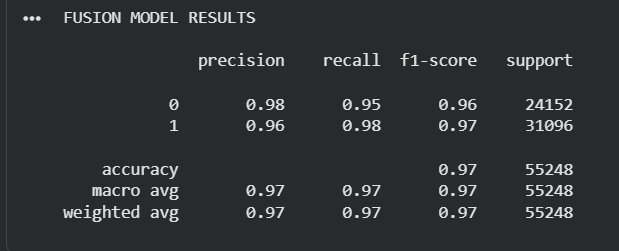
\includegraphics[width=0.80\textwidth]{Fusion_Model/Classification Result.png}
  \caption{Fusion Model classification results summary}
  \label{fig:fusion_result}
\end{figure}

\subsection{Fusion Model Confusion Matrix}

\begin{figure}[H]
  \centering
  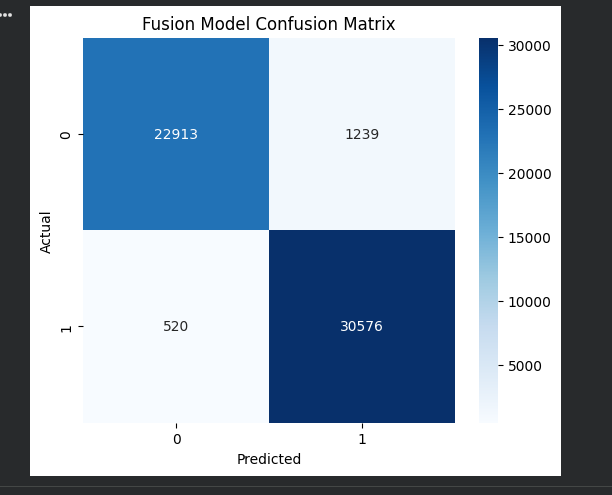
\includegraphics[width=0.75\textwidth]{Visualizations/Fusion Model Confusion Matrix.png}
  \caption{Fusion Model confusion matrix on the zero-day test set}
  \label{fig:fusion_cm}
\end{figure}

\noindent Breaking down the 55,248 test samples:
\begin{itemize}
  \item True Normals correctly classified: \textbf{22,913}
  \item Normal samples misclassified as Attack (false positives): \textbf{1,239}
  \item Zero-day Attacks correctly detected: \textbf{30,576}
  \item Zero-day Attacks missed (false negatives): \textbf{520}
\end{itemize}

\section{Model Comparison}

\subsection{Quantitative Comparison}

\begin{table}[H]
\centering
\caption{Comparison of all evaluated models}
\label{tab:model_comparison}
\begin{tabular}{llcc}
\toprule
\textbf{Model} & \textbf{Purpose} & \textbf{Accuracy} & \textbf{Zero-Day Capable} \\
\midrule
Isolation Forest (baseline) & Anomaly detection & 49.00\%  & Yes \\
LightGBM                    & Known attack clf  & 99.99\%  & No \\
Autoencoder                 & Zero-day detection & 99.19\% & Yes \\
\textbf{Fusion Model}       & \textbf{Hybrid}   & \textbf{96.82\%} & \textbf{Yes} \\
\bottomrule
\end{tabular}
\end{table}

\subsection{Performance Metric Comparison Chart}

\begin{figure}[H]
  \centering
  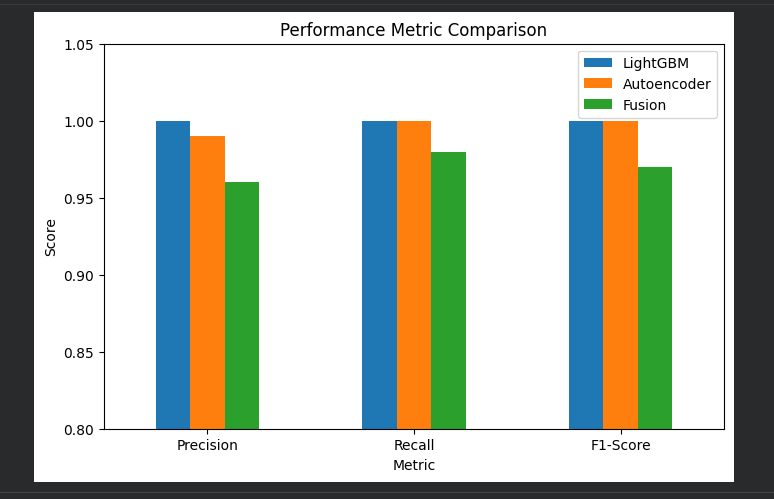
\includegraphics[width=0.85\textwidth]{Visualizations/Performance Metric Comparison.png}
  \caption{Performance metric comparison across all models}
  \label{fig:perf_comparison}
\end{figure}

\subsection{Zero-Day Detection Accuracy Comparison}

\begin{figure}[H]
  \centering
  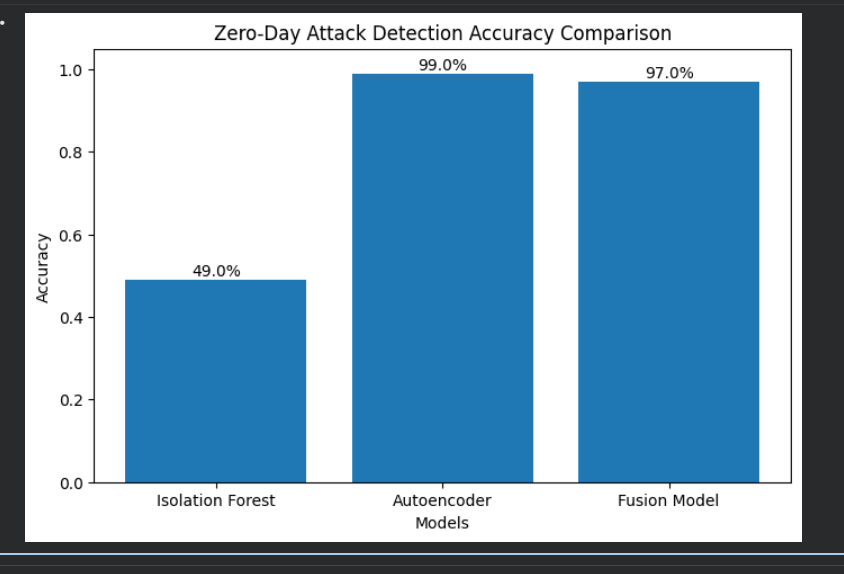
\includegraphics[width=0.85\textwidth]{Visualizations/Zero Day Attach detection Accuracy Comparison.png}
  \caption{Zero-day attack detection accuracy comparison}
  \label{fig:zeroday_comparison}
\end{figure}

\noindent The Isolation Forest baseline, despite being an unsupervised anomaly
detector, achieves only 49\% accuracy — barely above random chance — due to the
highly imbalanced nature of the dataset and the complex multi-modal distribution
of IoT attack traffic. In contrast, the Fusion Model achieves 96.82\%, a
\textbf{47.82 percentage-point improvement} over the baseline.

\section{Feature Importance Analysis}

The top features identified by LightGBM are presented below:

\begin{table}[H]
\centering
\caption{Top 10 features by LightGBM importance score}
\label{tab:feature_importance}
\begin{tabular}{lc}
\toprule
\textbf{Feature} & \textbf{Importance Score} \\
\midrule
tcp.srcport         & 13,467 \\
tcp.options         & 12,777 \\
tcp.dstport         & 8,849 \\
tcp.ack             & 7,849 \\
tcp.ack\_raw        & 6,417 \\
tcp.checksum        & 6,109 \\
tcp.seq             & 4,226 \\
http.request.method & 2,213 \\
tcp.len             & 2,181 \\
udp.stream          & 2,009 \\
\bottomrule
\end{tabular}
\end{table}

\noindent TCP-level features dominate the importance rankings, consistent
with the fact that most attacks in the dataset exploit TCP-based protocols.
Notably, 14 features (primarily ARP, MQTT metadata, and DNS fields) scored
zero importance, indicating they contribute no discriminative information
for the 10 known attack classes.



% ============================================================
%  CHAPTER 6 – DISCUSSION
% ============================================================
\chapter{Discussion}

\section{Key Findings}

\subsection{Effectiveness of the Hybrid Approach}

The experimental results confirm the central thesis of this project: a
hybrid system combining supervised classification and unsupervised anomaly
detection substantially outperforms either component alone when applied
to a zero-day detection scenario.

\noindent LightGBM, while achieving near-perfect accuracy (99.99\%) on
known attack categories, is completely blind to zero-day attacks — it can
only classify traffic into the 10 categories it was trained on. The
Autoencoder, trained on normal traffic, can detect any deviation from
normality regardless of the attack type, but it struggles to discriminate
between different attack categories. The Fusion Model inherits the strengths
of both: reliable known-attack classification and robust zero-day detection.

\subsection{Confidence-Based Routing}

The 90\% confidence threshold in the Fusion Model was empirically chosen to
minimise false negatives (missed attacks) while maintaining acceptable false
positive rates. A lower threshold would cause more traffic to be routed to
the Autoencoder, potentially increasing false positives on normal traffic.
A higher threshold would improve normal traffic precision but risk passing
subtle zero-day attacks through without Autoencoder scrutiny.

\subsection{Autoencoder False Positive Rate}

The Autoencoder's 5.13\% false positive rate on normal traffic is the
primary source of error in the Fusion Model. This is a known limitation of
reconstruction-error-based anomaly detection: certain normal traffic patterns
have high variance and produce reconstruction errors above the threshold.
Future work could address this by using a Variational Autoencoder (VAE) or
by incorporating class-conditional thresholds.

\section{Limitations}

\begin{enumerate}
  \item \textbf{Binary output}: The Fusion Model currently produces binary
        (Normal/Attack) output for zero-day traffic. It cannot identify which
        specific zero-day attack type has occurred.
  \item \textbf{Hardcoded paths}: All notebooks use Google Drive paths, limiting
        portability. Refactoring to relative paths would improve reproducibility.
  \item \textbf{Static threshold}: The anomaly threshold is fixed post-training.
        In a production system, it should be periodically updated as new normal
        traffic patterns emerge.
  \item \textbf{Zero-importance features}: 14 features with zero importance
        were retained in the final model. Pruning these would reduce model
        complexity without sacrificing accuracy.
  \item \textbf{Imbalanced classes}: Some attack categories have significantly
        fewer samples than others, which may cause the classifier to be biased
        towards majority classes.
\end{enumerate}

\section{Comparison with Related Work}

Compared to prior work using the Edge-IIoTset dataset or similar IoT
intrusion detection benchmarks:
\begin{itemize}
  \item \textbf{Ferrag et al.~\cite{dataset_edge_iiotset}} (dataset authors)
        evaluated several ML algorithms including Random Forest and Deep Learning
        on their dataset, reporting accuracies in the 95–98\% range on known attacks.
        Our LightGBM achieves 99.99\%, surpassing their best results.
  \item \textbf{Khraisat et al.~\cite{hybrid_survey}} surveyed hybrid IDS and
        found that the best hybrid systems achieved approximately 97–99\% accuracy
        on combined known/unknown attack scenarios. Our Fusion Model (96.82\%)
        is competitive with state-of-the-art hybrid approaches.
  \item The \textbf{Isolation Forest baseline} (49\% accuracy) confirms that
        naive unsupervised methods are insufficient for this domain, consistent
        with findings in the literature~\cite{iforest_limits}.
\end{itemize}

\section{Future Work}

Several directions are identified for future improvement:

\begin{enumerate}
  \item \textbf{Multi-class zero-day identification}: Train a second-level
        classifier on detected anomalies to identify zero-day attack families.
  \item \textbf{Online learning}: Implement incremental learning so the
        system can adapt its anomaly threshold to evolving traffic patterns
        without full retraining.
  \item \textbf{Variational Autoencoder}: Replace the standard Autoencoder
        with a VAE to obtain a probabilistic latent representation, enabling
        more principled anomaly scoring.
  \item \textbf{Feature selection}: Remove the 14 zero-importance features to
        reduce dimensionality and potentially improve generalisation.
  \item \textbf{Edge deployment}: Optimise the models (quantisation, pruning)
        for deployment on resource-constrained IoT gateway devices.
  \item \textbf{Real-time evaluation}: Extend the evaluation to a streaming
        environment using Apache Kafka or similar to measure latency
        and throughput.
\end{enumerate}



% ============================================================
%  CHAPTER 7 – CONCLUSION
% ============================================================
\chapter{Conclusion}

This project presented and implemented a \textbf{hybrid intrusion detection
system} for IoT networks that combines supervised and unsupervised machine
learning to detect both known and zero-day attacks. The system was evaluated
on the Edge-IIoTset dataset, a comprehensive real-world IoT network traffic
benchmark containing 15 attack categories.

\noindent The key contributions of this work are:
\begin{enumerate}
  \item \textbf{LightGBM classifier}: Achieves 99.99\% accuracy on 10 known
        attack categories, surpassing prior work on the same dataset.
  \item \textbf{Autoencoder anomaly detector}: Trained exclusively on normal
        traffic, it detects all attack types with 100\% recall and 99.19\%
        overall accuracy.
  \item \textbf{Fusion Model}: Integrates both components via a confidence-based
        routing strategy, achieving 96.82\% accuracy on a combined test set
        that includes five never-before-seen zero-day attack categories —
        a 47.82 percentage-point improvement over the Isolation Forest baseline.
\end{enumerate}

\noindent The results validate the hypothesis that combining supervised and
unsupervised techniques produces a system that is both highly accurate on
familiar threats and capable of detecting novel ones. The confidence-based
routing mechanism provides an elegant and computationally efficient integration
strategy that avoids running both models on every sample.

\noindent Future work will focus on multi-class zero-day attribution, online
threshold adaptation, and deployment of the optimised model on resource-constrained
IoT gateway hardware. The source code, trained model artefacts, and experimental
notebooks are available in the project repository at:
\url{https://github.com/shahiil-ahmed/zero-day-iot-project}

% ============================================================
%  BIBLIOGRAPHY
% ============================================================
\bibliographystyle{IEEEtran}
\bibliography{references}

\end{document}
